\documentclass[conference]{IEEEtran}
\IEEEoverridecommandlockouts

\usepackage{cite}
\usepackage{amsmath,amssymb,amsfonts}
\usepackage{algorithmic}
\usepackage{graphicx}
\usepackage{textcomp}
\usepackage{xcolor}
\usepackage{booktabs}
\usepackage{multirow}
\usepackage{array}
\usepackage[
    colorlinks=true,
    linkcolor=blue,
    citecolor=blue,
    urlcolor=blue
]{hyperref}

\def\BibTeX{{\rm B\kern-.05em{\sc i\kern-.025em b}\kern-.08em
    T\kern-.1667em\lower.7ex\hbox{E}\kern-.125emX}}

\begin{document}

\title{Distributional Pedagogical Alignment:\\An Evidence-Centered Framework for Knowledge Tracing}

\author{%
\IEEEauthorblockN{Author One}
\IEEEauthorblockA{\textit{Department of Computer Science} \\
\textit{University Name}\\
City, Country \\
author1@university.edu}
\and
\IEEEauthorblockN{Author Two}
\IEEEauthorblockA{\textit{Department of Computer Science} \\
\textit{University Name}\\
City, Country \\
author2@university.edu}
}

\maketitle

\begin{abstract}
Knowledge Tracing (KT) models a learner's evolving knowledge state from historical interactions to predict future performance. Recent work on KT has advanced in three directions, among others: richer interaction representations, distributional and uncertainty-aware knowledge states, and reasoning or interpretability mechanisms. We take an evidence-centered view of this task: an interaction supports a knowledge update only after it has been aggregated and interpreted under a pedagogical lens. We treat this interpretation as an explicit intermediate stage rather than leaving it as an implicit update computation. We propose a framework organized into four representation spaces: Interaction, Distribution, Knowledge, and Prediction. At its core is the \emph{Distributional Pedagogical Alignment} (DPA) module: interaction representations are projected into a distributional space, where learning patterns, which are structurally consistent across learners, are constructed and aligned with pedagogical principles. This yields the evidence that drives the knowledge-state update. The alignment operates on distributional patterns through soft pedagogical rules, so the representation is shaped by pedagogical theory rather than gradient descent alone. This paper presents the framework and its rationale as a conceptual foundation for ongoing research on evidence-centered knowledge tracing.
\end{abstract}

\begin{IEEEkeywords}
Knowledge Tracing, Evidence-Centered Design, Learning Pattern, Distributional Representation, Pedagogical Alignment
\end{IEEEkeywords}

% ====================================================================
\section{Introduction}
\label{sec:intro}

Knowledge Tracing (KT) models a learner's evolving knowledge state from learning interaction history to predict future outcomes~\cite{corbett1994kt, piech2015dkt}. Recent KT models have advanced interaction representation, uncertainty modeling, and reasoning, each in complementary ways~\cite{li2025mckt, xia2025cmdkt, chen2025ukt, li2025keenkt, wu2026sskt, nakagawa2019gkt, zhou2024psikt, hooshyar2026nskt, wu2026plkt}. Educational measurement theory views the task as inference from evidence: a learner's proficiency is not directly observable and must be inferred from observations. A measurement model characterizes the ``weight and direction'' of the evidence these observations carry about proficiency~\cite{mislevy2005ecd}. Formative assessment reinforces this view by treating each interaction as evidence to be elicited, interpreted, and used to inform instructional decisions~\cite{black2009formative}. This evidence-centered view serves as the fundamental principle of the proposed framework: an interaction does not directly alter knowledge but contributes to an update only after being aggregated and interpreted through a pedagogical lens.

Concretely, the proposal introduces an explicit layer, \emph{Distributional Pedagogical Alignment} (DPA), between the interaction representation and the mastery update, whose task is to interpret the evidence before it is used. This layer (i)~projects interactions into a distributional space and organizes them into \emph{learning patterns} that carry pedagogical meaning, (ii)~aligns those patterns with pedagogical principles, and (iii)~keeps the pattern structure consistent across learners. We organize the overall framework around this layer as four representation spaces with distinct roles: Interaction, Distribution, Knowledge, and Prediction (Figure~\ref{fig:framework}).

The contribution of this paper is threefold. First, a \emph{perspective}: it frames the knowledge update as an act of interpreting evidence, grounded in pedagogical theory. Second, a \emph{core mechanism}, \emph{Distributional Pedagogical Alignment}, that gives this interpretation an explicit stage of its own, aligning learning patterns with pedagogical principles in a distributional space. Third, an \emph{architecture} that organizes the framework into four representation spaces.

% ====================================================================
\section{Related Work and Positioning}
\label{sec:related}

Recent KT research follows three complementary themes. \textbf{Interaction representation} enriches interaction encoding with question semantics, difficulty, and knowledge-component (KC) topology~\cite{li2025mckt, xia2025cmdkt}. \textbf{Distributional and uncertainty-aware representation} models the knowledge state, or the concepts, as distributions rather than fixed points, which gives a vocabulary for confidence and similarity that point representations lack~\cite{chen2025ukt, li2025keenkt, wu2026sskt}. \textbf{Reasoning and interpretability} makes inference more transparent through graph-based, probabilistic, or neural-symbolic reasoning~\cite{nakagawa2019gkt, zhou2024psikt, hooshyar2026nskt, wu2026plkt}.

\smallskip\noindent\textbf{Positioning.} The framework centers on one mechanism: an explicit, differentiable alignment of learning patterns with pedagogical principles, placed between the interaction representation and the mastery update. The patterns are structured consistently across learners, so a single principle applies to every history. The alignment shapes them before any mastery is inferred. Prior KT models perform this evidence-interpretation step implicitly, entangle it with the mastery update, or do not formulate it from a pedagogical standpoint. Our proposal is to make this stage explicit and semantically meaningful, and to endow it with pedagogical constraints.

The mechanism integrates the three themes. It encodes interactions with KC topology, builds patterns in a distributional space, and refines them with a soft, principle-guided adjustment. Each ingredient is established: distributional mastery representations~\cite{zhou2024psikt,wu2026plkt,li2025keenkt}, pattern pooling~\cite{wu2026plkt}, and pedagogically informed modeling~\cite{hooshyar2026nskt}. The novelty lies in their interpretation as an explicit alignment stage.

Among these, PLKT~\cite{wu2026plkt} is the closest prior work, as it also reasons from patterns to outcomes. It assembles patterns directly from raw interaction history as temporal sliding windows and matches them to the target outcome. The proposed framework instead organizes patterns by pedagogical operators and aligns them against pedagogical principles. LPKT~\cite{shen2021lpkt} is close from a different angle, as it models the learning process directly with explicit learning and forgetting gates, but it does not construct learner-consistent patterns or a distributional evidence stage. These models are alternative design choices for individual components and form the comparison set for the planned evaluation (Section~\ref{sec:eval}).

% ====================================================================
\section{Problem Formulation}
\label{sec:formulation}

A learner's interaction history is a sequence $S_T=\{(q_t,r_t)\}_{t=1}^{T}$, where $q_t$ is the question (item) attempted at step $t$ and $r_t \in \{0,1\}$ indicates an incorrect/correct response. The KT task is to predict $\hat{y}=P(r_{t+1}=1 \mid q_{t+1}, S_T)$. The domain's knowledge structure is a set of knowledge components (KCs) $\mathcal{C}=\{c_1,\dots,c_C\}$, a question-to-KC mapping, and a knowledge graph $\mathcal{G}$ encoding heterogeneous relations (e.g., prerequisite, neighboring, applying) among KCs, read by the pattern constructor of Module~2. We treat $\mathcal{G}$ as a given, validated input, and leave learning the topology itself as a promising extension~\cite{wu2026sskt}.

The framework threads a learner's history through four representation spaces, introduced with each module in Section~\ref{sec:framework}; we leave the transformation equations to our future implementation paper. We use \emph{evidence} for the distributional representation in the alignment layer \emph{after} it has been pooled into patterns and pedagogically adjusted: a post-alignment object. A \emph{learning pattern} is the output of a fixed aggregation operator, defined by the aggregation rather than by the number of interactions it draws on.

% ====================================================================
\section{Proposed Framework}
\label{sec:framework}

\begin{figure*}[!htbp]
\centering
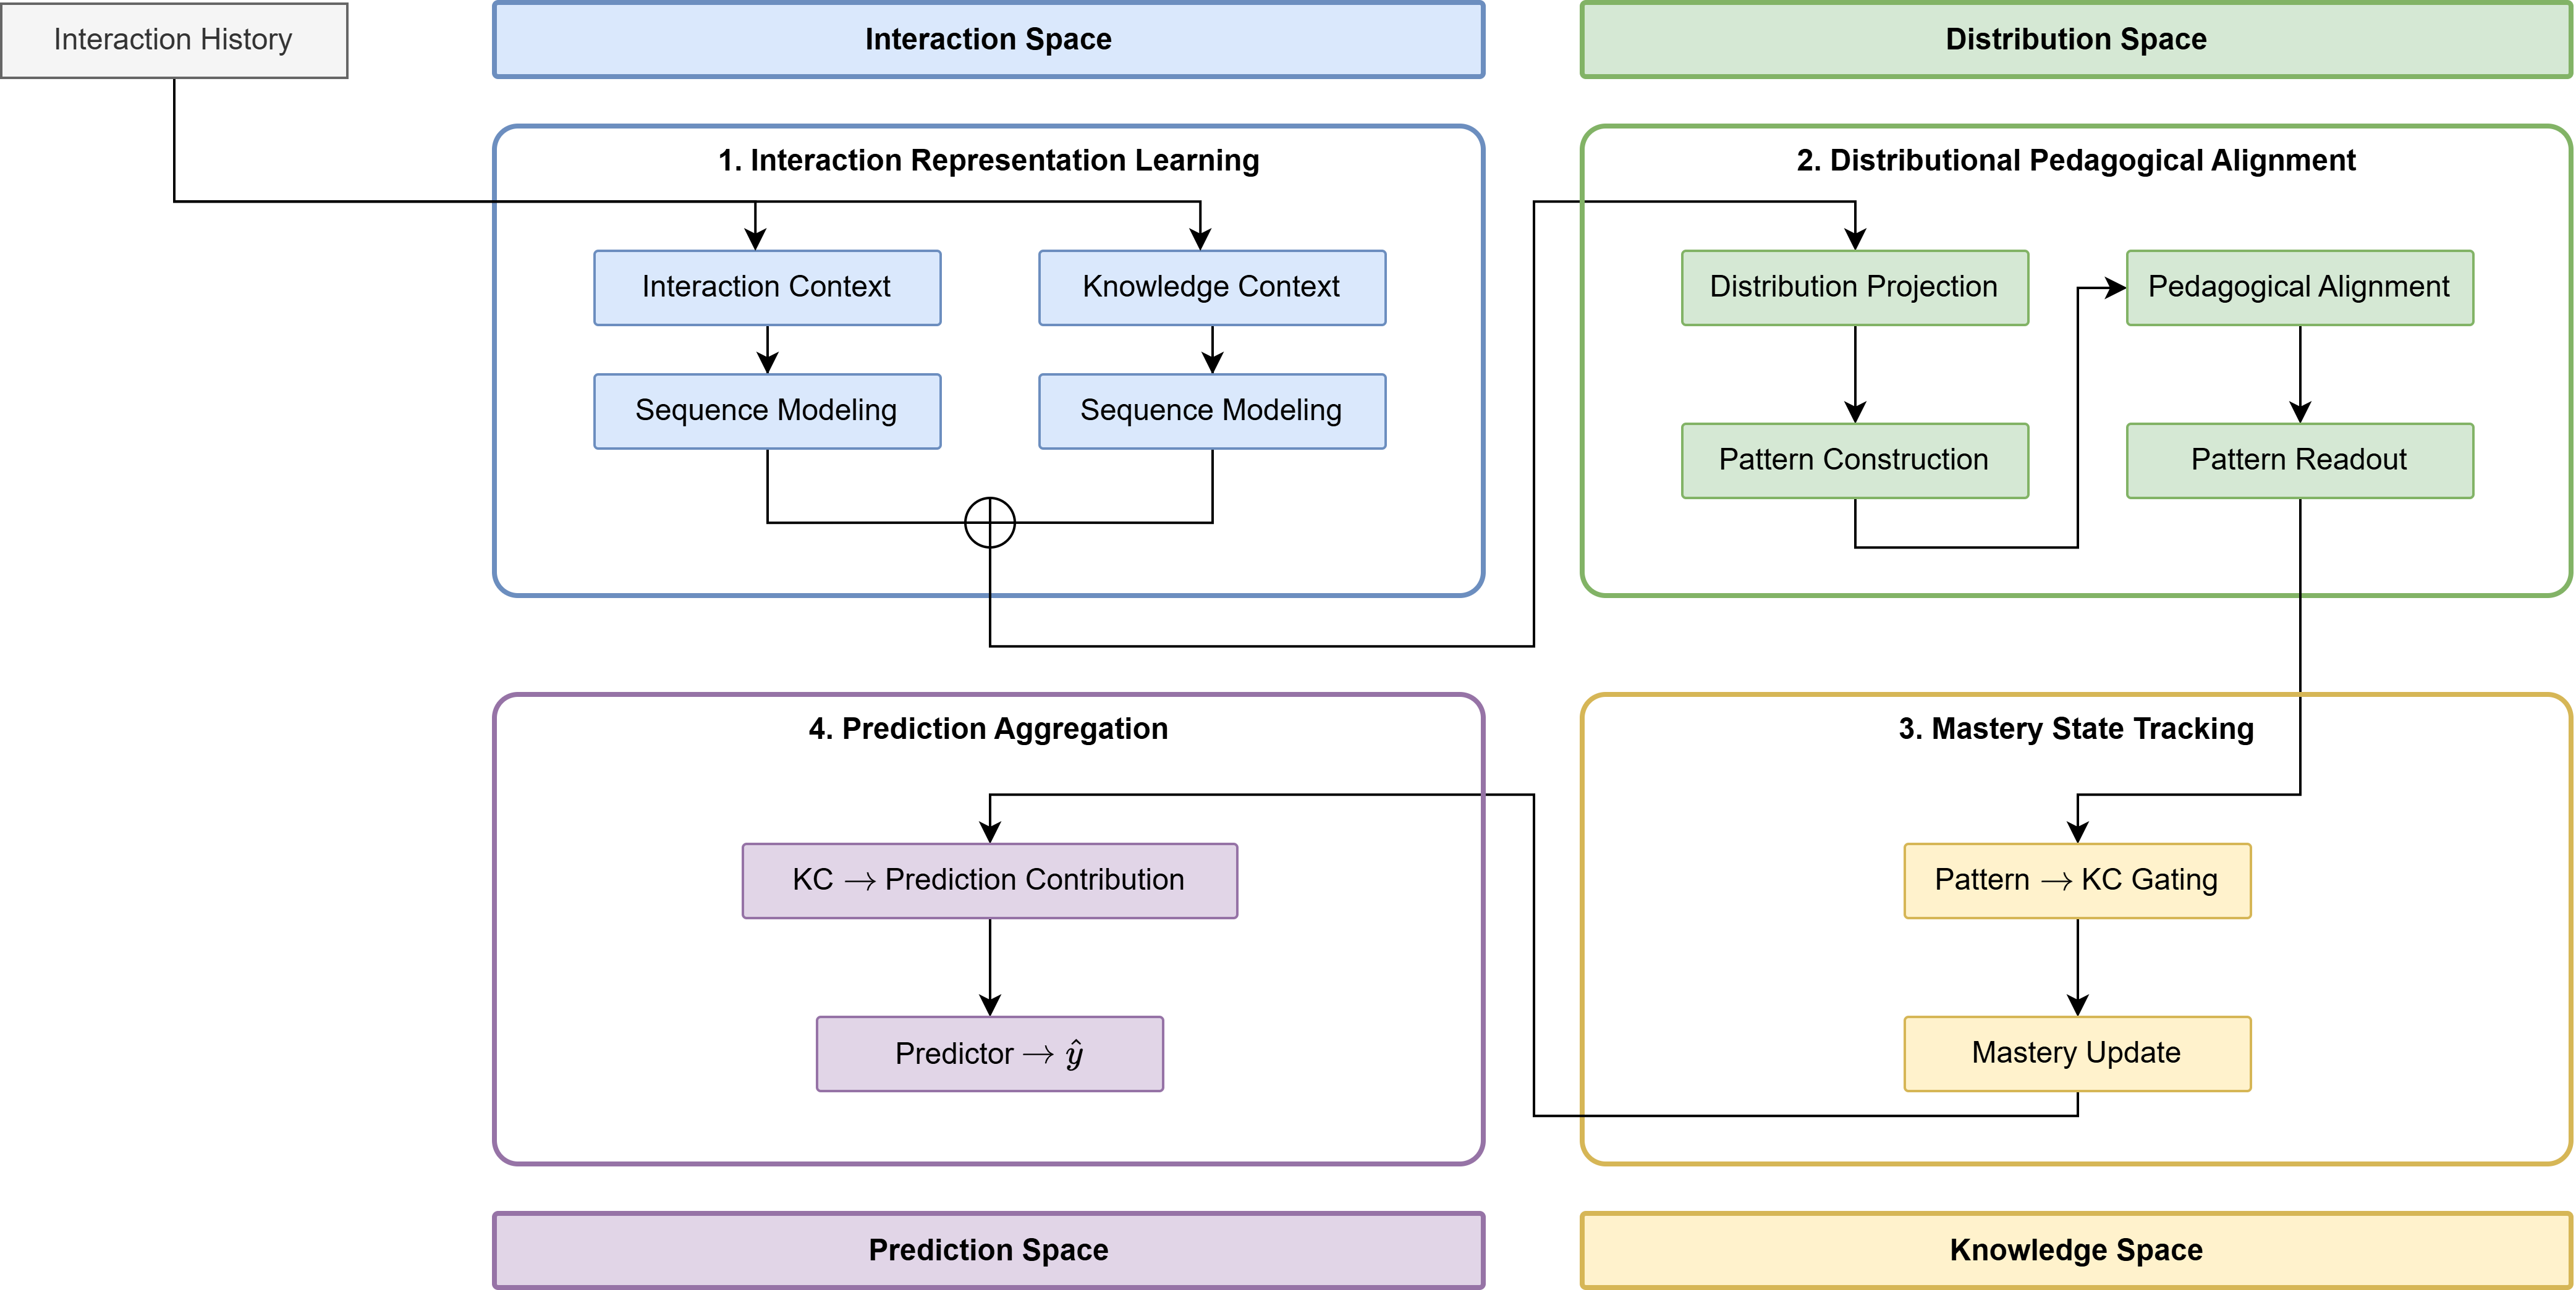
\includegraphics[width=0.92\textwidth]{framework}
\caption{Framework overview. Four modules over four representation spaces (color-coded). Evidence is \emph{produced} in Module~2, the mastery state is \emph{updated} in Module~3, and the prediction is formed in Module~4. Modules~3 and~4 additionally expose the pattern-to-KC contribution and the KC-to-prediction contribution, while Module~2 provides the learning patterns. The mastery memory is a per-learner recurrent state $M \in \mathbb{R}^{C \times d}$ over the $C$ knowledge components. At step $t$, Module~1 reads $M_{t-1}$ and Module~3 writes $M_t$.}
\label{fig:framework}
\end{figure*}

\subsection{Design Rationale: From Principle to Architecture}
\label{sec:rationale}

Evidence-centered design separates three kinds of models~\cite{mislevy2005ecd}. A ``student model'' carries the proficiency estimate. An ``evidence model'' turns observations into evidence. A ``task model'' specifies the tasks that produce those observations, together with their features and difficulty. The proposed spaces follow these models. \emph{Interaction} holds the observation, which is the learner's response to a given item. \emph{Distribution} is the evidence model, where observations are pooled into patterns and aligned into evidence. \emph{Knowledge} is the student model, which the gated update advances. The task model corresponds to the given task structure: the question and concept difficulty, the knowledge-graph topology, and the question-to-KC mapping. Knowledge tracing receives this structure rather than designing it, so it enters the framework as a fixed input. \emph{Prediction} is an added space that maps the student model to the next-step outcome.

The spaces also form a \emph{chain of preconditions}, in which each stage enables the next. A distributional representation preserves a dispersion that a point vector discards, so pooling retains how concentrated the evidence is. Pattern structure consistent across learners makes pedagogical alignment well-posed, because a shared principle needs a shared coordinate. And the explicit knowledge state then lets the update attribute evidence to specific KCs.

\subsection{Overview}

Figure~\ref{fig:framework} illustrates the framework, which comprises four sequential modules, one per space, and each realizing that space's role in the preconditional chain stated above. Module~1 learns the interaction representation. Module~2 turns that representation into a distributional one, pools it into learning patterns, aligns them with pedagogical principles, and reads out the structured evidence. Module~3 updates the explicit knowledge state from that evidence while learning a pattern-to-KC contribution. Module~4 aggregates the updated state with the target question to produce the prediction and a KC-to-prediction contribution.

\subsection{Module 1: Interaction Representation Learning}
\label{sec:irl}

The first module learns a contextual representation for each interaction from two input groups with distinct learning dynamics. The \emph{interaction context} gathers question semantics, the student response, and question difficulty. The \emph{knowledge context} combines a localized mastery representation with concept difficulty. The localized mastery is obtained by reading the previous step's mastery memory $M_{t-1}$ in the context of the current question via the knowledge graph. The two groups are processed by two parallel sequence-modeling branches: one capturing the dynamics of the interaction sequence, the other the dynamics of the local knowledge state. The two representations are fused into a single interaction representation.

\subsection{Module 2: Distributional Pedagogical Alignment}
\label{sec:dpa}

The alignment layer, DPA, proceeds in four conceptual steps:

\begin{enumerate}
    \item~\emph{Distribution projection} maps the interaction representation to a distributional one via a statistical-descriptor decoder. The decoder is a learnable map from the interaction representation to the statistical descriptors that define a distribution, such as its mean and variance. It carries the location and spread implicit in the interaction representation into an explicit distribution.
    \item~\emph{Pattern construction} builds several learning patterns using fixed pattern operators, so that each operator always carries the same pedagogical meaning and pattern structure is consistent across learners regardless of history length or distribution. A planned list of operators is: (i)~temporal pooling, which pools the most recent interactions; (ii)~same-KC pooling, which pools all interactions on the same KC; and (iii)~$\mathcal{G}$-aware pooling, which pools interactions following the KC topology.
    \item~\emph{Pedagogical alignment} aligns the patterns with pedagogical principles. Crucially, this alignment does not directly infer mastery. Instead, it nudges the patterns toward those principles as a soft, differentiable adjustment. A planned list of principles is:
    \begin{itemize}
        \item \emph{Guessing and slipping} emerge from the pattern representation. When patterns of the same KC and similar difficulty observe an outlier response, we consider the outlier a possible signal of guessing or slipping. The distributional pattern is then adjusted through its expectation and variance to absorb such possibilities.
        \item \emph{Monotonicity} acts as a debiasing prior on time gaps. Datasets record time gaps but cannot observe learner activity between interactions, such as review sessions, instructor guidance, or self-study. Treating a time gap as direct evidence of forgetting therefore injects a dataset-specific bias. The principle mitigates this in two ways. When the gap is large, but correctness is stable or rising, mastery is not reduced. When the error rate dips immediately after a gap and then returns to its prior level, the transient improvement is treated as slipping rather than a genuine gain, and mastery is not adjusted downward on that basis.
    \end{itemize}
    \item~\emph{Pattern readout} maps the aligned patterns back to a structured representation $z'$, in which each block corresponds to one pattern type. The readout preserves the statistical descriptor (i.e., the mean and variance) to carry over into the mastery update.
\end{enumerate}

\subsection{Module 3: Mastery State Tracking}
\label{sec:mst}

The third module maintains an explicit knowledge state and updates it from the structured pattern representation. Because the readout preserves the statistical descriptor, the update is uncertainty-weighted: evidence with higher variance yields a smaller mastery increment. Alongside the update, it learns a \emph{pattern-to-KC gating} that quantifies how much each learning pattern contributes to each related KC, and the state advances by a residual increment.

\subsection{Module 4: Prediction Aggregation}
\label{sec:pred}

The final module predicts the outcome of the next interaction from the updated knowledge state and a representation of the target question. Alongside the probability, it produces a \emph{KC contribution} (contribution of each KC to the target interaction) and forms the final prediction.

% ====================================================================
% ====================================================================
\section{Planned Evaluation}
\label{sec:eval}

\textbf{Datasets.} We plan to work in the mathematics domain, where the concept structure the pedagogical operators rely on is best established. Datasets are organized by whether that structure is available natively. Some benchmarks ship a genuine graph or tree, such as Junyi Academy~\cite{chang2015junyi}, XES3G5M~\cite{liu2023xes3g5m}, and Eedi/NIPS34~\cite{wang2021neurips}. Others are widely used flat-tag benchmarks, such as ASSISTments~\cite{feng2009assistments} and Algebra/Bridge-to-Algebra~\cite{stamper2010kddcup}, which we retain for scale and comparability. For the flat-tag benchmarks, we construct a graph following the validated procedure of CMDKT~\cite{xia2025cmdkt} and treat it as a fixed input (Section~\ref{sec:formulation}).

\textbf{Baselines.} For comparability, we build on the pyKT\footnote{\url{https://pykt.org/}} benchmark~\cite{liu2022pykt}. We compare against the foundational BKT~\cite{corbett1994kt} and against representatives of the three themes of Section~\ref{sec:related}. These span classic and attention-based deep KT (DKT~\cite{piech2015dkt}, DKVMN~\cite{zhang2017dkvmn}, AKT~\cite{ghosh2020akt}), graph- or representation-enriched models (GKT~\cite{nakagawa2019gkt}, CMDKT~\cite{xia2025cmdkt}), distributional models (UKT~\cite{chen2025ukt}, KeenKT~\cite{li2025keenkt}, S\textsuperscript{2}KT~\cite{wu2026sskt}), reasoning or pattern-based models (PSI-KT~\cite{zhou2024psikt}, NSKT~\cite{hooshyar2026nskt}, PLKT~\cite{wu2026plkt}), and learning-process models with explicit forgetting (LPKT~\cite{shen2021lpkt}, MemoryKT~\cite{lin2025memorykt}).

\textbf{Metrics and Ablations.} We report the standard AUC, accuracy, and RMSE. We add expected calibration error (ECE) and negative log-likelihood (NLL) to probe the distributional components. We plan three ablations: (i)~replacing the distributional representation with a point vector, (ii)~removing the alignment step, and (iii)~enabling the pattern operators one at a time. These probe the distributional space, the pedagogical alignment, and the pedagogically structured patterns. They are the elements of the precondition chain of Section~\ref{sec:rationale} that can be removed independently.

\textbf{Hypotheses.} We expect four outcomes. (H1)~The framework is competitive with strong baselines and improves most where a reliable concept structure lets the pedagogical operators contribute. (H2)~The relative gains are largest in data-scarce regimes, where learning patterns and pedagogical priors act as regularizers. (H3)~The pedagogical modules contribute positively in ablation, and the alignment adjustment shows behavioral consistency with the pedagogical rules. (H4)~Performance degrades gracefully as the concept structure is made noisier.

\smallskip\noindent\textbf{Potential for Interpretability.} The pattern-to-KC contribution and KC-to-prediction contribution can also be chained into a model-level attribution trace read from the model's own forward pass. We treat this only as an optional direction, not a contribution of the present design. Attention- or gating-style weights are not guaranteed to be explanations of the internal mechanism~\cite{jain2019attention,wiegreffe2019attention}, so we frame any such reading as behavioral consistency with pedagogical rules rather than a claim about the model's internals. A dedicated evaluation is left to future work.

\section{Conclusion}
\label{sec:conclusion}

We have presented a perspective on knowledge tracing in which updating knowledge is the interpretation of evidence, realized through an explicit intermediate layer, DPA, that pools interactions into learning patterns whose structure is consistent across learners and aligns them with pedagogical principles prior to mastery update. The framework's central addition is exactly DPA: the pedagogical alignment of learning patterns. As an ongoing research effort, our immediate research goals are to implement the framework and evaluate it on the benchmarks outlined in Section~\ref{sec:eval}; to study mechanisms that encourage the intended role separation; and to relax the knowledge graph toward a learnable topology.

% ====================================================================
% References
% ====================================================================
\bibliographystyle{IEEEtran}
\bibliography{references}

\end{document}
